\chapter{Survey}

\label{Chapter2}

\lhead{Chapter 2. \emph{Survey}}

This chapter will present the application case and the available data, discuss some important identity issues, and survey relevant research within the areas relevant to answering the research questions.

\section{The application case}
\label{survey:application_case}

  This section will introduce the application case, appear.in. First, to understand why it is of particular interest to study it, we need some context.

  \subsection{The modern web}
  \label{survey:the_modern_web}

    When we say that web applications are nearing the power and feature parity of traditional desktop applications, we are of course talking about the introduction of HTML5.

    HTML was originally designed as a language for describing scientific documents, and little more. Through the last decade, however, the concept of web applications slowly established itself, while lacking clear standardization efforts from the W3C. The HTML5 specification is an attempt to remedy this, by providing standards and guidelines for the browser vendors on how to implement a wide range of common APIs~\cite{W3CHTML5_intro}.

    In practice, these APIs lets websites do things like:

    \begin{itemize}
        \item play audio and video\footnote{\url{http://dev.w3.org/html5/spec-author-view/video.html}}
        \item generate graphics\footnote{\url{http://www.w3.org/TR/2dcontext/}}
        \item access your webcam and microphone\footnote{\url{http://www.w3.org/TR/mediacapture-streams/}}
        \item handle and manipulate arbitrary files\footnote{\url{http://www.w3.org/TR/FileAPI/}}
        \item send and recieve data over full-duplex socket connections\footnote{\url{http://www.w3.org/TR/websockets/}}
    \end{itemize}

    ...as well as a wide range of other things. In general, HTML5 enables web applications to do most of the things one would need plugins or native applications for just a few years ago.

  \subsection{The WebRTC specification}
  \label{survey:webrtc}

    One of the major HTML5 API specifications is called WebRTC\footnote{Web Real-Time Communication.}, and it is the last piece of the API puzzle enabling applications like appear.in.

    As the name implies, WebRTC handles real-time communication, but for the case of appear.in, an important aspect is that it is able to do so peer-to-peer. Although designed to be a protocol for exchanging arbitrary data between peers, it is particularly geared toward multimedia. For instance, the traditionally cumbersome task of setting up a two-way audiovisual connection is now a matter of dropping around 40 lines of boilerplate Javascript into a web page\footnote{For an excellent introduction, see: \url{http://www.html5rocks.com/en/tutorials/webrtc/basics/}.}.

    Although the WebRTC specification at the time of writing still officially is a working draft in the W3C\footnote{The latest specification can be found here: \url{http://dev.w3.org/2011/webrtc/editor/webrtc.html}.}, most of the large browser vendors have already implemented it. Consequentially, a plethora of applications leveraging this technology are already available, with ever more being launched every month.

  \subsection{Introducing appear.in}
  \label{survey:introducing_appearin}

    The main idea behind appear.in is simple enough: a conversation happens between users who are in the same room at the same time. The central idea, though, is that the \emph{conversation} is identified solely by the URL in use, and not in any way by the peers connecting. There is no notion of \emph{calling} someone -- you simply meet up in a room and talk. As an example, if any two people are visiting \url{https://appear.in/ntnu} at the same time, they will see and hear each other and can start chatting away.

    This view of a conversation as not really being an enitity in its own right, but rather an \emph{effect} of people being in the same room at the same time, breaks with the traditional model of audiovisual communication. Traditionally, talking to someone not present has been a process of one person \emph{calling} the other one, with group conversations usually being nothing more than an extension of this concept. appear.in doesn't concern itself with distinguishing between callers and callees, has no simple concept of a ``conversation'', and generally does not enforce any particular way of using the service -- apart from requiring the conversation venue, the ``room'', to be identifiable by a string of characters.

    Until the arrival of appear.in, this particular way of thinking about audiovisual conversations hadn't been a commonly seen pattern. However, the simplicity of the room concept opens the service up for a wide variety of uses: in addition to traditional video calls, we've already seen it used for everything from virtual offices and team meeting rooms to baby monitoring and remote tutoring, just to name a few.

  \subsection{The inner workings of appear.in}
  \label{survey:appearin_details}

  This section will pick apart the workings of appear.in to allow for a thorough understanding of what kind of an application we are dealing with. This should provide a good basis for understanding the generated data and the applicability of the results for the general case.

    As illustrated in figure~\ref{fig:appearin_arch}, the appear.in architecture is quite simple. It is built on a simple peer-to-peer (P2P) architecture, with signaling done through a centralized service endpoint.

    \begin{figure}[h]
      \centering
        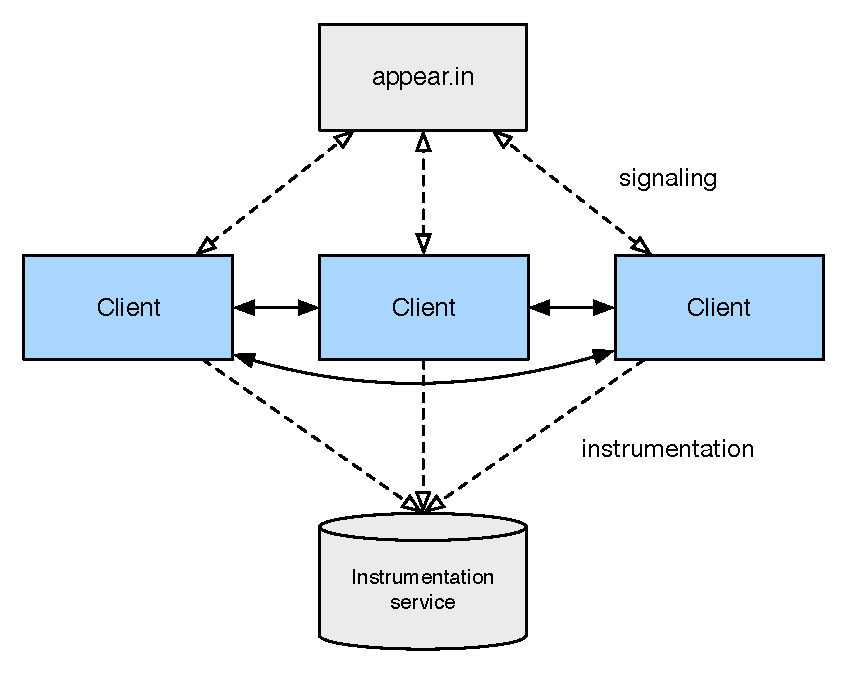
\includegraphics[width=0.9\textwidth]{Figures/appearin-arch}
        \caption{The appear.in architecture, illustrated for a conversation between 3 peers. \\ The black arrows indicate media data flow, and the dashed arrows indicate metadata flow: signaling data and instrumentation data, respectively.}
        \label{fig:appearin_arch}
    \end{figure}

    The instrumentation service has been included simply to illustrate the fact that the available data is generated and logged \emph{directly from the clients}.

    By ``signaling'', in the context of appear.in, we mean everything not directly related to the media streams between the peers. This includes:

    \begin{itemize}
      \item Managing which peers are in which room.
      \item Setting up new peer connections when a client joins a room.
      \item Tearing down peer connections when a client exits a room.
      \item Distributing various metadata that needs to be in sync across peers.
    \end{itemize}

    The user interface is also quite simple. It consists of a landing page (a screenshot of the current version can be seen in figure~\ref{fig:appearin_landing}), and a ``room page'' (see figure~\ref{fig:appearin_room}). For the sake of simplicity, let's go through them separately.

    \subsubsection{The landing page}

    \begin{figure}[h]
      \centering
        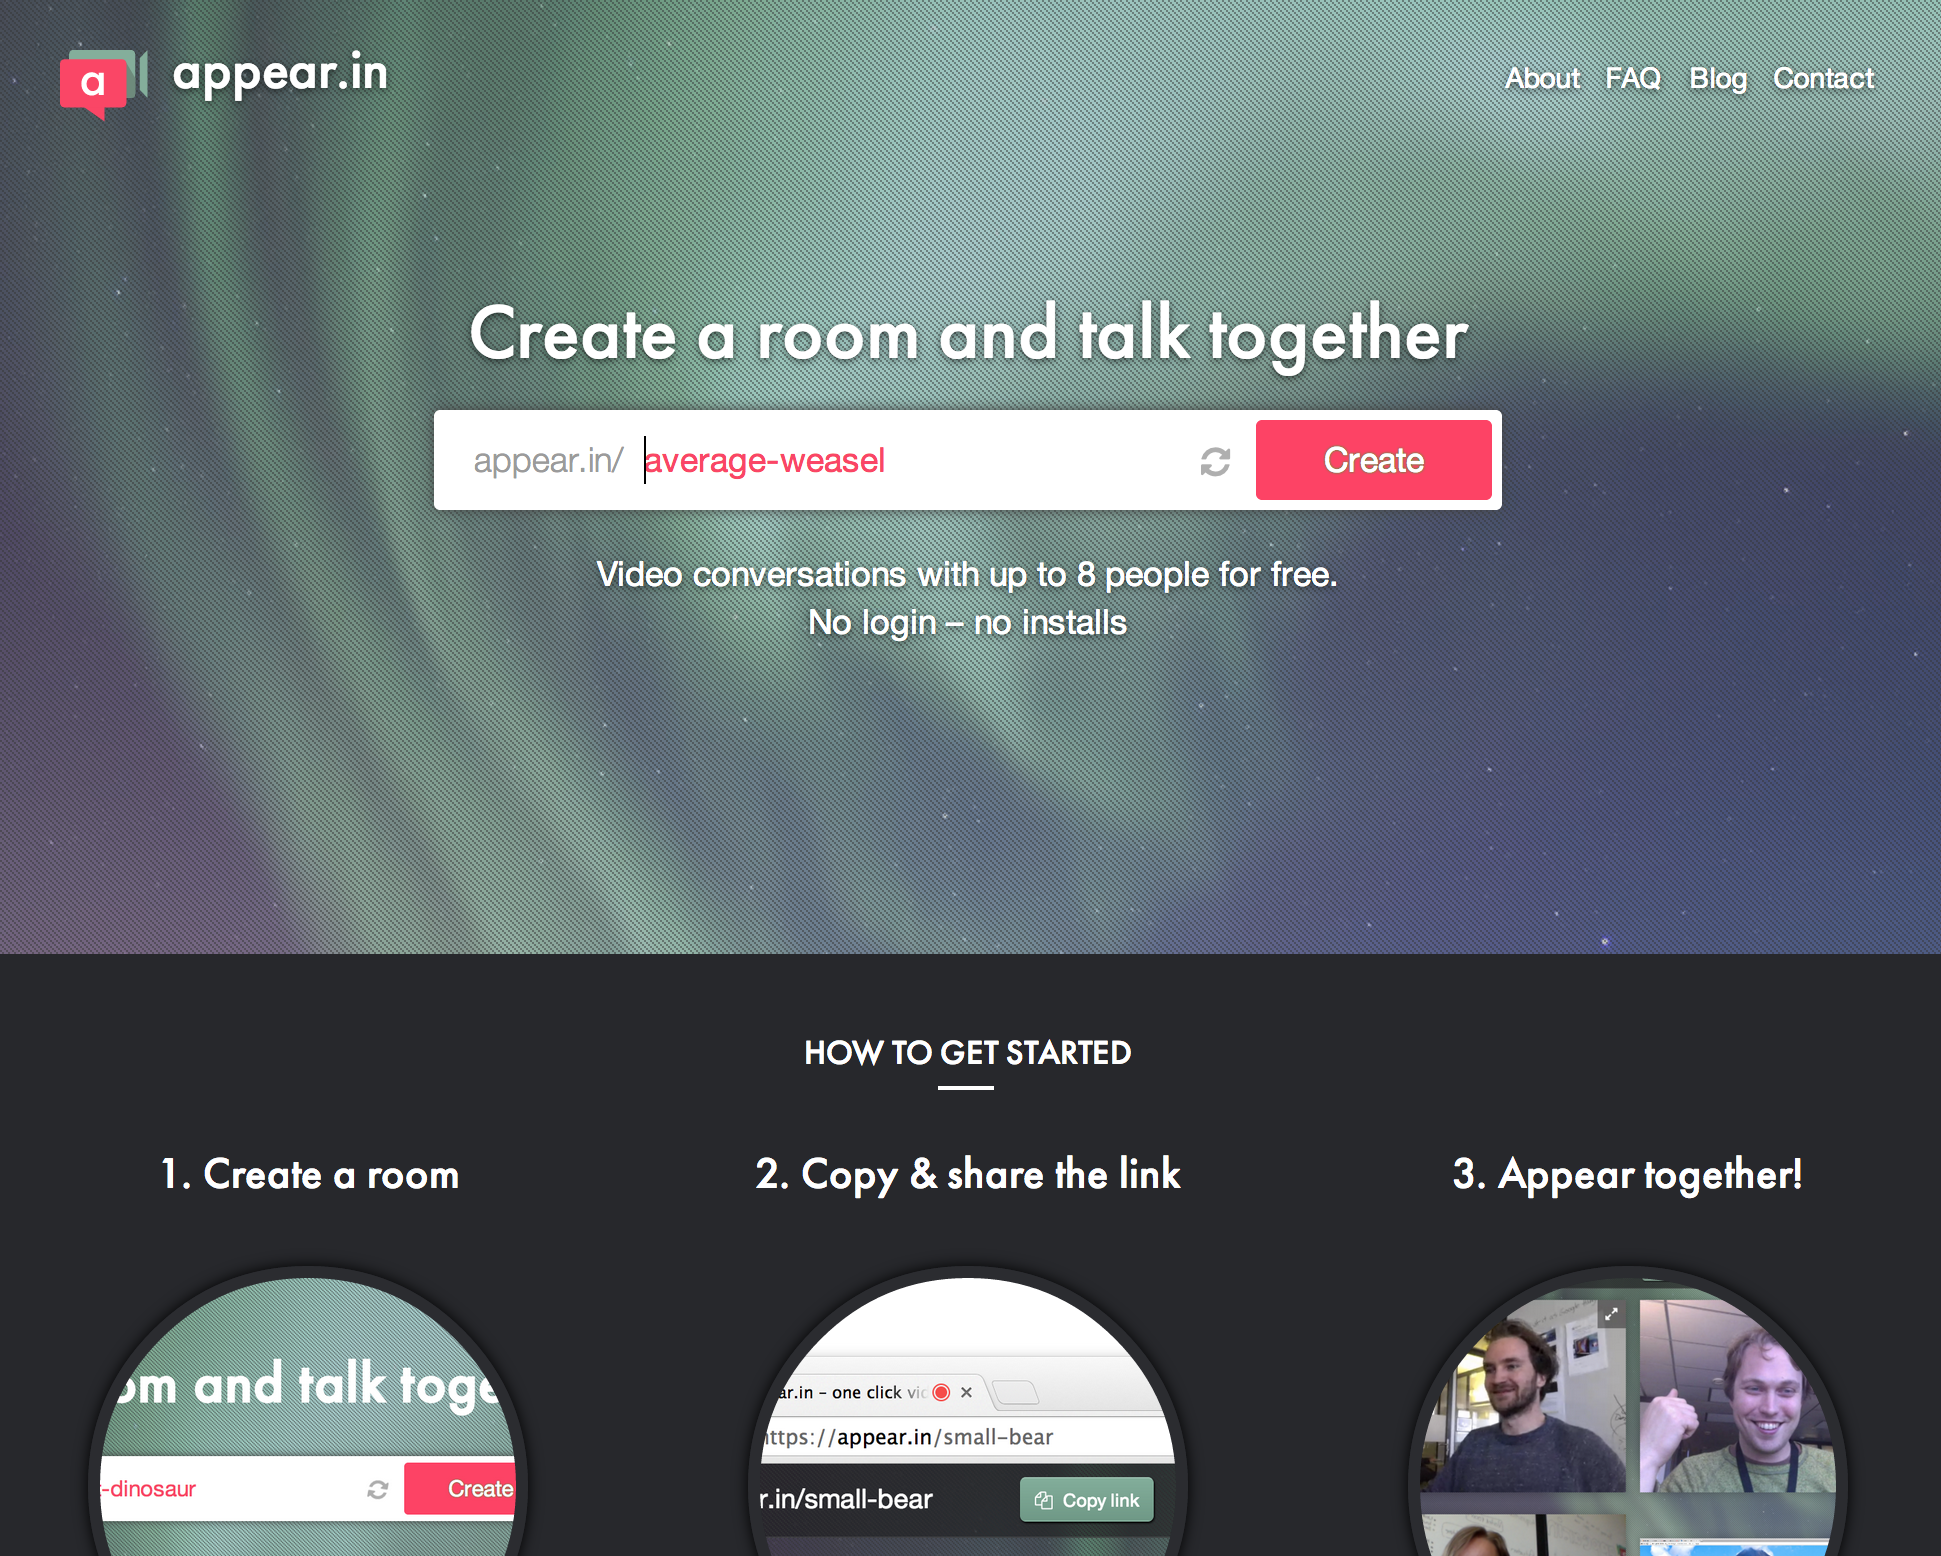
\includegraphics[width=\textwidth]{Figures/screenshots/appearin/frontpage-v2}
        \caption{The appear.in landing page (as of \today).}
        \label{fig:appearin_landing}
    \end{figure}

    The landing page's objective, as for most landing pages, is two-fold: to \emph{evoke interest}, and to \emph{activate the user}. Although we cannot directly measure them, we can indirectly measure the degree of interest and the activation rate in two ways:

    \begin{enumerate}
      \item The ratio of users going from the landing page to a room (interest).
      \item The ratio of users going from the landing page to a room to a conversation (activation).
    \end{enumerate}

    The concept of evoking interest and of activating the user are universal terms that should generalize well to many other web applications.

    \subsubsection{The room page}

    \begin{figure}[t]
      \centering
        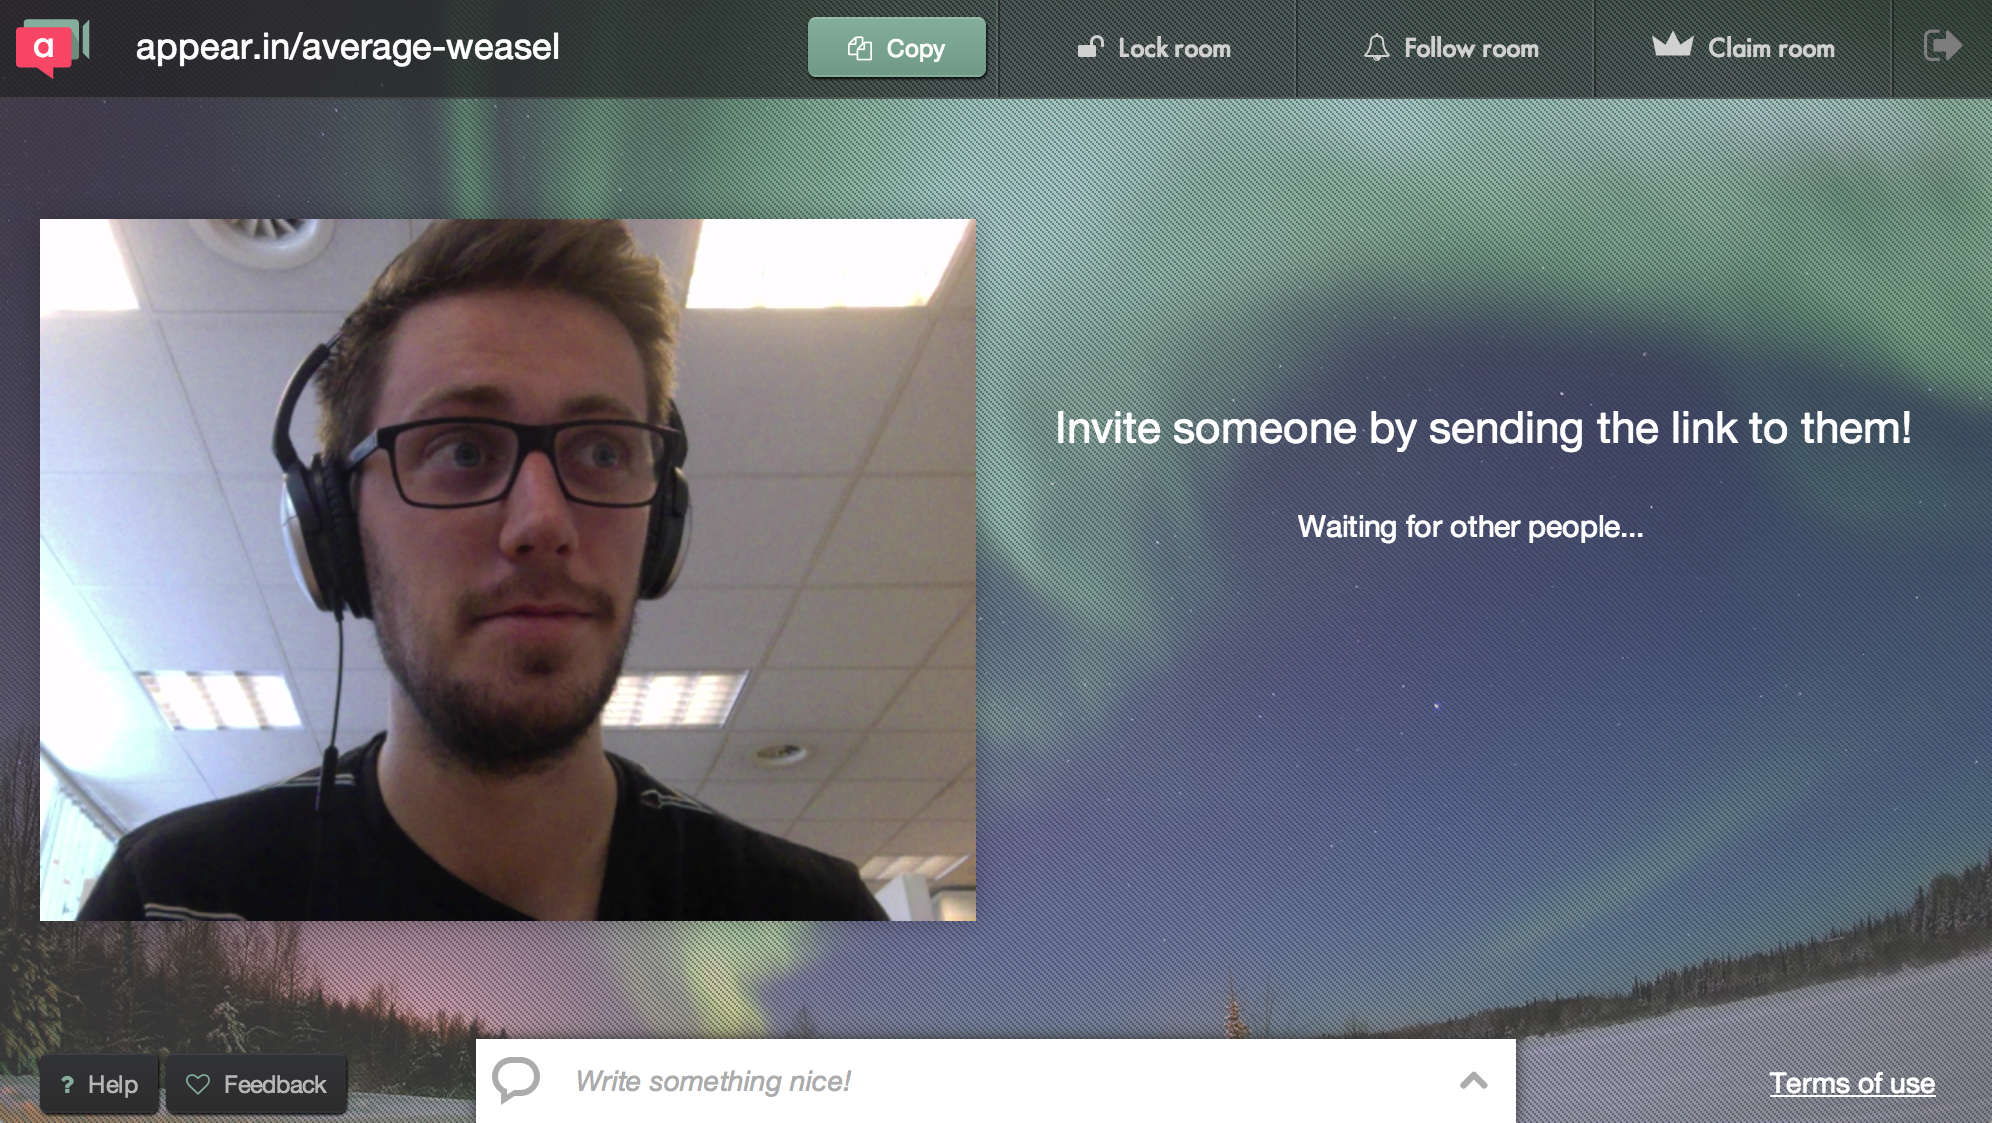
\includegraphics[width=\textwidth]{Figures/screenshots/appearin/in-room}
        \caption{The author in an appear.in room (as of \today).}
        \label{fig:appearin_room}
    \end{figure}

    The room page, the actual product user interface, is composed of several parts. Each participant resides in his or her own video control, and various room controls are placed along the top and bottom parts of the page.

    As the quality of the video conferencing part of the application is largely governed by the browser and other low-level technicalities, we will mostly focus our efforts on the functionality augmenting the content: effectively, the rest of the UI.

    The leftmost part of the top bar consists of a URL copying control, as shown in figure~\ref{fig:ui:copy_control}. Many users utilize this area when copying the page URL to invite their peers to the room. However, seeing as the same effect is easily achieved by copying the address field of the browser -- which we cannot track -- use of this control does not give a complete picture of users' sharing behavior.

    To the top right is a row of buttons, as shown in figure~\ref{fig:ui:top_buttons}. Respectively, they allow the user to ``lock'', ``follow'', ``claim'', and leave the room. Of these, only the first three are of particular interest, as the ``leave room'' button essentially does nothing but close the window, severing the connection.

    All these buttons alter the state of the room. Let's briefly walk through them.

    \begin{description}
      \item[Lock] \hfill \\
        When locking a room, one prevents other people who stumble upon the room's URL from entering.\footnote{They are, however, able to knock their way in, much in the same fashion as one would enter a locked room in the physical world.}
      \item[Follow] \hfill \\
        Users following a room are notified when other people enter it. A room's followers may also follow the room chat without being present in the room, by using a browser extension.
      \item[Claim] \hfill \\
        Users can claim a previously unclaimed room, and essentially take ownership of it. This enables them to customize the room in a number of ways.
    \end{description}

    The last piece of the feature puzzle is the chat control, depicted in figure~\ref{fig:ui:chat}. When users post a message, it becomes visible to other members. Chat messages are written to a centralized store, and persist as long as there are people in the room.

    \begin{figure}[t]
      \centering
      \begin{subfigure}[t]{0.8\textwidth}
        
\includegraphics[width=\textwidth]{Figures/screenshots/appearin/feature-copy}
        \caption{The room URL copying control.}
        \label{fig:ui:copy_control}
      \end{subfigure}

      \vspace{.5cm}

      \begin{subfigure}[t]{0.95\textwidth}
        
\includegraphics[width=\textwidth]{Figures/screenshots/appearin/feature-buttons-top}
        \caption{The top button row. Each button serves its own purpose and fires its own event.}
        \label{fig:ui:top_buttons}
      \end{subfigure}

      \vspace{.5cm}

      \begin{subfigure}[t]{0.95\textwidth}
        
\includegraphics[width=\textwidth]{Figures/screenshots/appearin/feature-chat}
        \caption{The chat control.}
        \label{fig:ui:chat}
      \end{subfigure}

      \caption{The most important UI parts.}
      \label{fig:important_ui_parts}
    \end{figure}


\section{The quality of the data}
\label{survey:data_quality}

  As shown in figure~\ref{fig:appearin_arch}, the clients send various data to an external instrumentation service. While the details of the instrumented data are discussed in section~\ref{approach:sub:generating_data}, this section will deal with the general quality of the clients as a data source.

  \subsection{Lack of demographics}
  \label{survey:lack_of_demographics}

    A key facet of all user adaptation and personalization is adapting to a user's interests, and so it is imperative to learn about the user. Montgomery and Srinivasan introduce a distinction between active and passive learning to aid in categorizing approaches to the issue~\cite{Montgomery2002}. Whereas active learning results from direct questions to the user, passive learning is the opposite: learning about the user without asking.

    Active learning has several disadvantages in the general case:

    \begin{enumerate}
      \item It requires too much effort on the customer's part.
      \item The user may indeed not know the answer to the questions, either lacking the proper knowledge or experience to evaluate the alternatives.
      \item The user may be unwilling to reveal correct answers.
      \item It is inefficient, as it typically ignores information consumers reveal about their preferences in their past interactions and purchases.
    \end{enumerate}

    The first point applies especially to the case of appear.in. An important part of the product is the simplicity of the application, ie. the small amount of friction. Thus, introducing questionnaires or similar approaches to collecting active feedback from users has not been viewed as a positive tradeoff up to this point.

    So, we will be limited to passive learning. What does this leave us with in practice?

    Montgomery identifies three major sources of information from which it is possible to learn passively: transaction data, clickstream data, and email.

    appear.in, being a so-called single-page web application (SPA), has no clickstream in the traditional sense, a traditional clickstream being the series of pages navigated to. Transactional data, on the other hand, is usually related to e-commerce, and to some sense of ``items bought''. This is similarly irrelevant in this particular interpretation. However, we \emph{can} choose to view the series of interactions with the application as a clickstream of sorts -- an event stream -- and use it as a data source in much the same way.

  \subsection{What is a user identity?}
  \label{survey:identity}

    Before moving on, let's define some words and concepts that will be central to this section, and to the rest of the thesis. The following definitions have been taken from the Merriam-Webster online dictionary\footnote{\url{http://www.merriam-webster.com/dictionary/}}.

    \begin{description}
      \item[Anonymous] \hfill \\
        Lacking individuality, distinction, or recognizability.
      \item[Pseudonymous] \hfill \\
        Using a pseudonym: a name that someone uses instead of his or her real name.
      \item[Identity] \hfill \\
        The distinguishing character or personality of an individual.
    \end{description}

    Adapted to our realm, this thesis will use these words in the following ways.

    \begin{description}
      \item[Anonymous] \hfill \\
        Not being recognizable as a person from the collected user data.
      \item[Pseudonymity] \hfill \\
        Being able to identify users without actual personal information.
      \item[Identity] \hfill \\
        The qualities that allow us to distinguish users from each other.
    \end{description}

    In these word senses, appear.in is an anonymous communication service: no personal information is ever collected about the users, and not even IP-addresses or geolocational data is logged on an individual level. By tracking individual \emph{browsers} using cookies, however, we can track users -- or more precisely, browsers -- over time.

    By logging various events that we deem interesting along with a cookie value identifying the browser, we can reconstruct user sessions, and connect them to the application users pseudonomously.
    % By ``pseudonomously'' it is meant that we identify the users solely by a random string set in their browser.

  \subsection{Client-side identity}
  \label{survey:client_side_identity}

    Several others have written about how privacy constraints impact personalized systems~\cite{Teltzrow2004,Kobsa2007}. Indeed, the very nature of anonymity is an extension of privacy. However, the absence of \emph{identity} presents an entirely different challenge when designing personalization systems.

    There are ways of coping with the absence of user identification. Kobsa, for instance, describes an approach that makes heavy use of pseudonyms designed around this problem~\cite{Kobsa2003}. However, user pseudonyms in appear.in -- the tracking cookies -- reside only in the user's browser, and may be lost at any time.

    This all makes tracking users very problematic. However, we can somewhat circumvent the problem using web cookies, albeit with a very time-limited effect.

    \subsubsection{Unstable user state with cookies}
    \label{survey:state_with_cookies}

      The first time a user visits appear.in, a cookie is set with a \emph{random value} uniquely identifying the \emph{browser}. It is this value which is sent with every event to the instrumentation service, as described in figure~\ref{fig:appearin_arch}.

      Unfortunately, using only cookies for identification has its clear downsides. Should the user clear the browser cache, switch browsers, use the browser ``incognito''\footnote{Google lingo for private browsing, where previously set cookies are not available (among other things).}, or simply use multiple machines, then different user ids will be generated and used in each case.

      As we shall see, most users periodically clear their browser cookies (see~\ref{survey:privacy_vs_personalization} for numbers), which causes an abrupt end of the perceived event stream from the browser user, never to be reassumed. The effect is illustrated in figure~\ref{fig:clear_cookie_impact} for a hypothetical case, in which user $A$ clears the browser cache twice, effectively cutting off the event stream each time. There is no obvious way to consolidate the three event streams of the three perceived users $A$, $B$, and $C$.

      Without tracking more user information -- IPs and locations, for instance -- there is no easy way of tying these user ids together, to reason about them as a single user. However, collecting this information about users goes against appear.in's privacy policy, and it has been deemed more interesting to see what can be done without crossing this line.

      \begin{figure}[h]
        \centering
          \begin{subfigure}[t]{0.8\textwidth}
            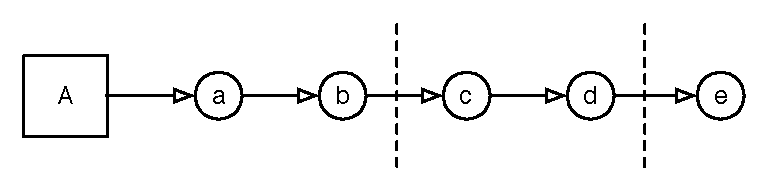
\includegraphics[width=\textwidth]{Figures/event-flow-cache-break-1}
            \caption{An event flow from $a \rightarrow e$, as seen from a user $A$. The dashed vertical lines indicate a point at which the user clears the browser cache.}
            \label{fig:cache_break1}
          \end{subfigure}
          \begin{subfigure}[t]{0.8\textwidth}
            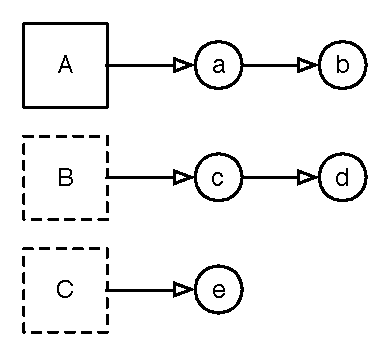
\includegraphics[width=0.5\textwidth]{Figures/event-flow-cache-break-2}
            \caption{The same event flow as perceived by the system.}
            \label{fig:cache_break2}
          \end{subfigure}

          \caption{The impact that clearing the browser cookies has on the chronological event stream for a single user $A$.}
          \label{fig:clear_cookie_impact}
      \end{figure}

      In practice, this leads to sparse usage data and quite a bit of noise in the event stream used as the basis for the user model generation.
      % Furthermore, the shortening of event streams also introduces a bias to the clustering algorithms, as the user model vectors will be shorter than is actually the case.

  \subsection{Privacy versus personalization}
  \label{survey:privacy_vs_personalization}

    There are not only the technical sides of user tracking to deal with. Due to a wide range of non-technical reasons, there exists at the time of writing a great deal of controversy surrounding online privacy.

    This section discusses how this affects our current ability to perform effective user adaptations, and includes some prospects for the future.

    Teltzrow and Kobsa~\cite{Teltzrow2004} state our predicament plainly: ``Personalization systems need to acquire a certain amount of data about users' interests, behavior, demographics and actions before they can start adapting to them.'' As we shall see, many Internet users are highly sceptical of providing personal information to web sites, and a majority are concerned about web sites tracking their movements and behavior online. This doesn't fit adaptive systems' demand for data collection.

    \subsubsection{Personal information}

      First, consider the following survey results regarding personal infomation~\cite{Teltzrow2004}:

      \begin{enumerate}
        \item Internet Users who are concerned about the security of personal information: 83\%~\cite{CyberDialogue2001}, 70\%~\cite{Behrens2001}, 84\%~\cite{Fox2000}
        \item People who have refused to give (personal) information to a web site: 82\%~\cite{Culnan2001}
        \item Internet users who would never provide personal information to a web site: 27\%~\cite{Fox2000}
        \item Internet users who supplied false or fictitious information to a web site when asked to register: 34\%~\cite{Culnan2001}, 24\%~\cite{Fox2000}
      \end{enumerate}

      Although the above numbers aren't directly relevant to the case of appear.in, where no personal information is collected or stored, it underlines a general scepticism towards providing information to web sites.

      The fact that such a large portion of users are sceptical of providing personal data tells us that there is reason to believe there is room for anonymous niches within most application areas, serving as a drive towards more applications like appear.in.

    \subsubsection{Tracking}

      While there is no theoretical upper bound to the lifetime of a tracking cookie, surveys of Internet users, as well as our own analyses, see that they usually do not persist for very long~\cite{Teltzrow2004}:

      \begin{enumerate}
        \item People who are concerned about being tracked on the Internet: 60\%~\cite{CyberDialogue2001}, 54\%~\cite{Fox2000}, 63\%~\cite{Harris2000}
        \item Internet users who generally accept cookies: 62\%~\cite{PersonalizationConsortium2000}
        \item Internet users who set their computers to reject cookies: 25\%~\cite{Culnan2001}, 3\%~\cite{CyberDialogue2001}, 31\% in warning modus~\cite{CyberDialogue2001}, 10\%\cite{Fox2000}
        \item Internet users who delete cookies periodically: 52\%~\cite{PersonalizationConsortium2000}
      \end{enumerate}

      These numbers are backed up by looking at the decline over time of user cookies in appear.in, as shown in figure~\ref{fig:perceived_user_persistence}.

    \subsubsection{The road ahead}

      Although these numbers are a bit dated, there is little reason to believe that the tracking situation is going to get any easier in the years to come~\cite{RuizMartinez2012,Nikiforakis2013,Sorensen2013,Eijk2011}.

      As we have seen, there already exists broad scepticism towards the use of cookies to track users, even on first-party sites. Much of the problem seems to stem from sites allowing third-party cookies, to better serve advertisements to its users -- who often are oblivious to the tracking taking place at all.

      These third-party cookies, however, allow these third-parties to track users' activity and behavior across multiple sites, often without their explicit consent. This has recently been deemed as bordering to surveillance, and in recent years extensive legislative restrictions have been introduced to decrease the prevalence of particularly third-party cookies.

      This all presents a challenge for services like appear.in, who use third-party cookies not to advertise, but to enhance the service for the user. There is reason to believe this situation will not become easier to deal with in the years to come, but hopefully, there will come about better ways of dealing with the issue.

\section{Identifying stereotypes}
\label{survey:identifying_sterotypes}

  There are many approaches to the task of sterotyping users. In this project we will approach the task using clustering techniques.

  In the broad sense of the problem at hand -- adapting the application -- there are, of course, alternatives to the clustering approach. Two of them are \emph{classification} and \emph{collaborative filtering}~\cite{Mitchell1997}:

  \begin{description}
    \item[Collaborative filtering] \hfill \\
      Let us briefly reiterate on the first main research question: is it possible to consistently stereotype the users? While collaborative filtering may be a good approach to the user adaptation problem isolated, it will not be able to aid us in identifying stereotypes.
    \item[Classification] \hfill \\
      Classification problems require training sets with predefined classes. As there is no preexisting set of stereotypes, and no \emph{known} patterns within the data, a classification approach is unfeasible.
  \end{description}

  Due to these constraints, the clustering approach is chosen. The following sections take a closer look at how we can use clustering techniques to identify and evaluate the quality of user clusters.

  \subsection{Stereotyping with clustering techniques}
  \label{survey:clustering_intro}

    There are many different clustering models, and many distinctions that can be made between them. The following list contains a brief introduction of some of those most commonly used.

    \begin{description}
      \item[Centroid models] \hfill \\
        Each cluster is represented by a single vector, indicating its center.
      \item[Connectivity models] \hfill \\
        Typically hierarchical clustering, where models are built based on distance connectivity.
      \item[Density models] \hfill \\
        Defines clusters as dense areas in the data space.
    \end{description}

    The most common model by far is the centroid model, more specifically the k-means approach~\cite{Berkhin2006}. This is the clustering scheme to be used in the approach described in chapter~\ref{Chapter3}.

    The k-means algorithm has several strong suites with regard to our application~\cite{Berkhin2006}:

    \begin{enumerate}
      \item It is a good match with regard to both input and desired output for our data.
      \item The implementation used in this project, the Lloyd-Forgy algorithm~\cite{Forgy1965}, parallelizes and scales very well.
      \item Being the most commercially used clustering scheme, the results will more easily compare to those of other applications.
    \end{enumerate}

    The algorithm itself and its generated results are described in detail in~\ref{approach:clustering}.

  \subsection{Evaluating clusters}
  \label{survey:evaluating_clusters}

    In general, any clustering method should search for clusters whose members are close to each other and well separated. Berry and Linoff~\cite{Berry1996} formulate it in terms of \emph{compactness} and \emph{separation}.

    \begin{description}
      \item[Compactness] \hfill \\
        The members of each cluster should be as close to each other as possible.
      \item[Separation] \hfill \\
        The clusters themselves should be widely spaced.
    \end{description}

    For an algorithm such as $k$-means, which takes the $k$ as an input, the central question when it comes to cluster validity is for which value of $k$ the cluster compactness and separation are optimal.

    The most efficient way of measuring cluster quality between several executions of a clustering method, where only its parameters -- like $k$ -- differ, is to utilize a so-called \emph{relative criteria}~\cite{Halkidi2001}.

    One of the most widely used measures of clusters' relative criteria is the Davies-Bouldin index, which is the one used to differentiate between clusters in this project. It is defined as:

    \begin{equation}
      \text{DB}_k = \frac{1}{k} \sum_{i=1}^k \max_{j,\,i \neq j} \left( \frac{s_i + s_j}{d(c_i, c_j)} \right)
    \end{equation}

    where $k$ is the number of clusters, $c_x$ is the centroid of cluster $x$, $s_x$ is the average distance of all elements in cluster $x$ to centroid $c_x$, and $d(c_i,c_j)$ is the distance between centroids $c_i$ and $c_j$.

    In plainer words, the Davies-Bouldin index formulates a measure of the quality of cluster separation and compactness, while considering the number of clusters in a responsible manner. Thus, it is well suited to distinguish between runs of eg. the $k$-means algorithm, where the value of $k$ differs from run to run.

\section{Adaptive systems}
\label{survey:adaptive_systems}

  Adaptive systems have been around for quite some time, and they exist in many forms. This section will focus mainly on the subject of user modeling and adaptive graphical user interfaces.

  \subsection{History of user modeling}

    This historical dissertation is loosely based on Vrieze and Kobsa~\cite{Vrieze,Kobsa2001}.

    The first work within user modeling research was conducted in the nineteen-eighties. Strongly influenced by the field of artificial intelligence, the groundwork for modern user modeling was laid.

    The common denominator for the user modeling systems composed in this era was their tight integration with their respective production systems. The end of the era, however, saw systems such as GUMS~\cite{Finin1989}, the first standalone user modeling system. These early standalone systems are most widely known as User Modeling Shell Systems, a term coined by Kobsa in 1990~\cite{Kobsa1990}.

    The nineteen-nineties was a decade widely dominated by User Modeling Shell Systems, which carried on the tradition of GUMS from 1989. Mostly, stereotype-based approaches were used, which sought to deduce logical connections between user models and the application domain.

    One system, however, Doppelgänger~\cite{Orwant1995}, stands out in this regard, being the only system to employ a probabilistic model, and not a logic-based approach~\cite{Kobsa2001,Pohl1997,Pohl1999}.

    Into the new millenium, many systems began to leverage internet capabilities and were focused on the web. A special class of these systems are commercial user modeling systems. While their capabilities in terms of inference were limited, they provided other capabilities needed for commercial use. They offered features such as linking with external data sources and a client server architecture for scalability and flexibility.

    Much recent research has gone into adapting mobile devices, smart appliances and homes, and development of generic user modeling tool systems~\cite{Vrieze,Gajos2006,Findlater2008}.

  \subsection{Designing adaptive graphical user interfaces}

    As user modeling work often manifests itself as user interfaces, naturally, there has been done extensive work on how the answers provided from a user modeling system can be applied to an actual production system.

    This research area differs from the purely user modeling angle, as described in the previous section, in two important ways:

    \begin{enumerate}
      \item They tend to focus on ways of applying concrete interface adaptations, and their respective effects on actual users.
      \item The conclusions are often of qualitative nature, basing themselves on user testing.
    \end{enumerate}

    Results from this kind of research tends to measure an adaptation's success not in terms of transactions and ROI, but in terms of user satisfaction and the quality of the user experience~\cite{Gajos2006,Findlater2008}.

    As we shall see, the system described in this thesis is indeed inspired by this approach, particularly in its use of feature experiments to power user adaptations. We will come back to this point in section~\ref{approach:feature_experiments}.

  \subsection{State of the art}

    Adaptive user interfaces have not been commercially available for very long, at least not in the commercial application sphere. It is not many years since adaptive \emph{menus} first hit the mainstream, with Microsoft's Smart Menus\texttrademark\ and the various start menus that have been launched since Windows XP~\cite{Gajos2006}.

    On the other hand, when it comes to adaptive hypermedia, the main focus of research seems to be on eLearning~\cite{Vrieze}, and on adapting to different screen sizes and mobile devices~\cite{Findlater2008}.

    All these approaches, however, operate under non-restraining conditions.

    There has indeed been extensive research into consolidating privacy concerns and personalization~\cite{Kobsa2007,Wang2010,Wang2012,Knijnenburg2013}, but no significant research seems to have targeted the realm of personalizing strongly privacy-constrained web applications.
